% This must be in the first 5 lines to tell arXiv to use pdfLaTeX, which is strongly recommended.
\pdfoutput=1
% In particular, the hyperref package requires pdfLaTeX in order to break URLs across lines.

\documentclass[11pt]{article}

% Change "review" to "final" to generate the final (sometimes called camera-ready) version.
% Change to "preprint" to generate a non-anonymous version with page numbers.
\usepackage[final]{acl}

% Standard package includes
\usepackage{times}
\usepackage{latexsym}
\usepackage{comment}

% For proper rendering and hyphenation of words containing Latin characters (including in bib files)
\usepackage[T1]{fontenc}
% For Vietnamese characters
% \usepackage[T5]{fontenc}
% See https://www.latex-project.org/help/documentation/encguide.pdf for other character sets

% This assumes your files are encoded as UTF8
\usepackage[utf8]{inputenc}

% This is not strictly necessary, and may be commented out,
% but it will improve the layout of the manuscript,
% and will typically save some space.
\usepackage{microtype}

% This is also not strictly necessary, and may be commented out.
% However, it will improve the aesthetics of text in
% the typewriter font.
\usepackage{inconsolata}

%Including images in your LaTeX document requires adding
%additional package(s)
\usepackage{graphicx}
\usepackage{booktabs}
\usepackage{multirow}
\usepackage{xcolor}
\usepackage{hyperref}
\usepackage{amsmath}
\usepackage{mathtools}
\usepackage{makecell}
\usepackage{ltablex}
\usepackage{longtable}
\usepackage{supertabular,booktabs}
\usepackage{xltabular}
\usepackage{tikz}
\usepackage{pgfplots}
\usetikzlibrary{patterns}
\usepackage{xspace}
%\usepackage{numprint}
%\npdecimalsign{.}
\usepackage{booktabs,siunitx}
\usepackage{pgf-pie}

\sisetup{
  table-auto-round = true, % Round numbers in S-columns
  % detect-weight=true,
  detect-all = true,
  % detect-inline-weight=math
}

% If the title and author information does not fit in the area allocated, uncomment the following
%
%\setlength\titlebox{<dim>}
%
% and set <dim> to something 5cm or larger.

% \title{Faithful, Unfaithful or just Ambiguous? Multi-agent Summary Evaluation through Debate with Initial Stance}
% Faithful or not? Depends! Identifying ambiguity by taking a stance in multi agent debate
% \title{Improved Faithfulness Evaluation by Identifying Ambiguity and Taking a Stance in Multi-Agent Debate }
\title{Faithful, Unfaithful or Ambiguous? Multi-Agent Debate with Initial Stance for Summary Evaluation}
% Multi-agent Summary Evaluation through Debate with Initial Stance
% Multi-agent Debate with Initial Stance for Summary Evaluation
% \title{MADDISSE: Multi-Agent Debate with Initial Stance fro Summary Evaluation}

% Author information can be set in various styles:
% For several authors from the same institution:
% \author{Author 1 \and ... \and Author n \\
%         Address line \\ ... \\ Address line}
% if the names do not fit well on one line use
%         Author 1 \\ {\bf Author 2} \\ ... \\ {\bf Author n} \\
% For authors from different institutions:
% \author{Author 1 \\ Address line \\  ... \\ Address line
%         \And  ... \And
%         Author n \\ Address line \\ ... \\ Address line}
% To start a separate ``row'' of authors use \AND, as in
% \author{Author 1 \\ Address line \\  ... \\ Address line
%         \AND
%         Author 2 \\ Address line \\ ... \\ Address line \And
%         Author 3 \\ Address line \\ ... \\ Address line}

% \author{First Author \\
%   Affiliation / Address line 1 \\
%   Affiliation / Address line 2 \\
%   Affiliation / Address line 3 \\
%   \texttt{email@domain} \\\And
%   Second Author \\
%   Affiliation / Address line 1 \\
%   Affiliation / Address line 2 \\
%   Affiliation / Address line 3 \\
%   \texttt{email@domain} \\}

\author{
 \textbf{Mahnaz Koupaee\textsuperscript{1}\thanks{Work done as an intern at Amazon.}},
 \textbf{Jake W. Vincent\textsuperscript{2}},
 \textbf{Saab Mansour\textsuperscript{2}},
 \textbf{Igor Shalyminov\textsuperscript{2}},
\\
 \textbf{Han He\textsuperscript{2}},
 \textbf{Hwanjun Song\textsuperscript{3}},
 \textbf{Raphael Shu\textsuperscript{2}},
 \textbf{Jianfeng He \textsuperscript{2}},
\\
 \textbf{Yi Nian\textsuperscript{2}},
 \textbf{Amy Wing-mei Wong\textsuperscript{2}},
 \textbf{Kyu J. Han\textsuperscript{2}},
 \textbf{Hang Su\textsuperscript{2}},
\\
%  \textbf{Thirteenth Author\textsuperscript{3}},
%  \textbf{Fourteenth F. Author\textsuperscript{2,4}},
%  \textbf{Fifteenth Author\textsuperscript{1}},
%  \textbf{Sixteenth Author\textsuperscript{1}},
% \\
%  \textbf{Seventeenth S. Author\textsuperscript{4,5}},
%  \textbf{Eighteenth Author\textsuperscript{3,4}},
%  \textbf{Nineteenth N. Author\textsuperscript{2,5}},
%  \textbf{Twentieth Author\textsuperscript{1}}
% \\
\\
 \textsuperscript{1}Stony Brook University,
 \textsuperscript{2}Amazon,
 \textsuperscript{3}Korea Advanced Institute of Science and Technology
 % \textsuperscript{4}Affiliation 4,
 % \textsuperscript{5}Affiliation 5
\\
 \texttt{
   % \textbf{Correspondence:} 
   % \href{mailto:mkoupaee@cs.stonybrook.edu}
   mkoupaee@cs.stonybrook.edu
 }
}

\newcommand{\mk}[1]{\textcolor{violet}{$_{Mahnaz}${[#1]}}}
\newcommand{\hs}[1]{\textcolor{teal}{$_{Hang}${[#1]}}}
\newcommand{\sm}[1]{\textcolor{cyan}{$_{Saab}${[#1]}}}
\newcommand{\is}[1]{\textcolor{magenta}{$_{Igor}${[#1]}}}
\newcommand{\hh}[1]{\textcolor{gray}{$_{Han}${[#1]}}}
\newcommand{\jv}[1]{\textcolor{brown}{$_{Jake}${[#1]}}}
\newcommand{\rs}[1]{\textcolor{purple}{$_{Raphael}${[#1]}}}

\newcommand{\method}[0]{\textsc{Madisse}\xspace}

\begin{document}
\maketitle
\begin{abstract}
Faithfulness evaluators based on large language models (LLMs) are often fooled by the fluency of the text and struggle with identifying errors in the summaries. %, usually leading to high false negative rate.
We propose an approach to summary faithfulness evaluation in which multiple LLM-based agents are assigned initial stances (regardless of what their belief might be) and forced to come up with a reason to justify the imposed belief, thus engaging in a multi-round debate to reach an agreement. The uniformly distributed initial assignments result in a greater diversity of stances leading to more meaningful debates and ultimately more errors identified.
Furthermore, by analyzing the recent faithfulness evaluation datasets, we observe that naturally, it is not always the case for a summary to be either faithful to the source document or not. We therefore introduce a new dimension, \textbf{\textit{ambiguity}}, and a detailed taxonomy to identify such special cases. Experiments demonstrate our approach can help identify ambiguities, and have even a stronger performance on non-ambiguous summaries\footnote{Code and data available at \href{https://github.com/amazon-science/madisse}{github.com/amazon-science/madisse}}.

%({\sc TofuEval}, {\sc LLM-AggreFact})
% LLM-based faithfulness evaluators are often fooled by the fluency of the text and struggle with identifying errors in the summaries, usually leading to high false negative rate.
%\is{We propose an approach to summary faithfulness evaluation in which multiple LLM-based agents are assigned initial stances (regardless of what their belief might be) and forced to come up with a reason to justify the imposed belief, thus engaging in a multi-round debate to reach an agreement. The uniformly distributed initial assignments here result in a greater diversity of stances leading to more meaningful debates and ultimately more errors identified.}
% We propose an approach in which multiple LLM-based agents are assigned initial stances (regardless of what their belief might be) and forced to come up with a reason to justify the imposed belief. 
% Then they engage in a multi-round debate to reach an agreement. 

%\is{Furthermore, by analyzing the recent faithfulness evaluation datasets ({\sc TofuEval}, {\sc LLM-AggreFact}), we observe that naturally, it is not always the case for a summary to be either unambiguously faithful to the source document or not.}
% However, we can only expect full agreement if we assume that the faithfulness of a summary \textsc{always} has a right answer and should be either categorized as faithful or unfaithful which might not be the case.
%A summary is ambiguous if it can be correctly interpreted in different ways and then can be seen as both faithful and unfaithful depending on the interpretation. In the setting of multiple raters, that leads to low inter-annotator agreement (IAA) and potentially erroneous conclusions regarding the system performance and ranking. We therefore introduce a new dimension \textbf{\textit{ambiguity}} and a detailed taxonomy to identify such special cases. 
%Our experiments demonstrate the following: first, how the debate approach can help with identifying more errors compared to the existing approaches; second, how the arguments generated in the debate can help with identifying ambiguous cases; and finally, how the debate approach can have even a stronger performance on non-ambiguous summaries.

% SM abstract:
% \sm{Faithfulness evaluation of abstractive summaries is traditionally constrained to the binary judgement of faithful or not faithful. This binary categorization fails to account for instances where ambiguity arises and the final judgment depends on underlying assumptions. The limited binary approach contributes to low inter-annotator agreement (IAA), leading to potentially erroneous conclusions regarding system performance and ranking. In this paper, we propose a novel approach to faithfulness evaluation by introducing an additional "ambiguous" category, accompanied by a detailed taxonomy of ambiguity types. To identify ambiguous cases, we employ a multi-agent debate framework, where agents are initialized with a stance. Our findings demonstrate that initializing agents with a stance not only improves the detection of ambiguous cases but also enhances the correlation between agents and human judgments. This approach offers a finer grained and more accurate method for evaluating faithfulness, leading to more reliable assessments of summarization systems.}

% \textbf{VERSION 1:}
% With the recent progress of LLMs, automatic summary evaluation using LLMs has gained a lot of attention to replace the costly human labor. However, they are far from perfect, struggling with capturing the subtle nuances of the LLM-generated summaries, often being fooled by the fluency of the text and therefore missing on a large proportion of existing errors.
% We propose a LLM-based multi-agent setup in which agents will engage in a debate based on their randomly assigned initial stance on the faithfulness of the summary, and try to convince each other. The initialization forces the agents to think out-of-box and deeper to identify aspects that would go unnoticed otherwise.  
% By inspecting the arguments from the debate approach, we observed the faithfulness should not be seen as a binary classification task and therefore we introduce a third dimension \textbf{\textit{ambiguity}} with a detailed taxonomy to account for cases where there are sound arguments for both faithfulness and unfaithfulness depending on how one would interpret the summary.
% We show that not only the debate approach can help identify more errors and the judgments to be better aligned with human annotations but also further show how the debate arguments can help identifying ambiguous cases. 

% \textbf{VERSION 2:} 
% Faithfulness evaluation of abstractive summaries is usually done by assessing whether a sentence is faithful or not but ignoring the fact the a summary sentence can be \textit{correctly} interpreted in different ways given the context and therefore can be evaluated as both faithful or unfaithful depending on the underlying assumptions.
% We therefore introduce a new dimension \textbf{\textit{ambiguity}} along with a detailed taxonomy of potential ambiguity types to account for cases which can have contrastive faithfulness labels depending on how one would interpret the summary. 
% We also propose a LLM-based multi-agent debate setup in which evaluator agents with random initial stance on the faithfulness of the summary engage in a multiple rounds of debate, trying to convince each other. 
% Our experiments show that not only can the proposed framework improve the overall performance of LLM-based evaluators, but also the final arguments by the evaluator agents can help identify the ambiguous cases.

\end{abstract}

\section{Introduction}
Summary evaluation has a long history, and over the years, different approaches have been applied to evaluate the quality of the generated summaries including n-gram based metrics \cite{lin2004rouge,papineni2002bleu}, representation-based approaches \cite{zhang2020bertscoreevaluatingtextgeneration}, finetuned specialized evaluators \cite{kryscinski2020evaluating,fabbri2022qafacteval,goyal2020evaluating,clark2023seahorse,tang2024minicheck} and human evaluation. 
With recent advancements in LLMs and their superior ability to generate fluent text, automatic summary evaluation has gained even more attention. In particular, assessing aspects like faithfulness has become more challenging due to the high fluency of LLM-generated text. 

While overlap-based metrics usually show weak correlation with human judgments \cite{liu2023g,tang2024tofueval} and finetuned approaches usually lack explainability, human evaluation is also costly with high turnaround time, low reproduciblity and low inter annotator agreement (IAA). With that said, efficient and accurate evaluation of summaries still remains a challenge. 

Automatic evaluation using LLMs have shown promising results, overcoming some of the major bottlenecks of traditional approaches in efficient evaluation of the generated summaries.
Different single-LLM and multi-LLM settings have been applied on a wide range of tasks and are shown to be strong automatic evaluators \cite{liu2023g,luo2023chatgptfactualinconsistencyevaluator,wang2023factcheck,chan2023chateval,song2024finesure}. 
% 
But even LLMs as evaluators fail to identify a large portion of the errors and are often fooled by the fluency of the LLM-generated summaries. 
Interestingly, when told that a given summary is unfaithful, LLMs can come up with correct reasoning and arguments that they couldn't otherwise, showing their inherent potential for error detection.
% \sm{TODO add citation}. 
To efficiently exploit the error detection capability of the LLMs to reason about the faithfulness of a given summary, we propose \textbf{\method}, a Multi-Agent Debate with Initial Stance for Summary Evaluation framework, in which LLM-based agents will be assigned opposing initial stances (either faithful or unfaithful) as their beliefs on the faithfulness quality of the summary. 
Forcing LLMs to come up with reasons to justify an initial stance might not always lead to correct prediction as the stances are random and might not be aligned with actual faithfulness labels.
Therefore, agents engage in multiple rounds of debate with each other, either support or refute others’ arguments with the aim of resolving any inconsistencies and reaching an agreement on the final label.

However, the main underlying assumption in faithfulness evaluation is that a summary \textsc{always} has a right answer and can either be classified as faithful or unfaithful which might not be the case. 
A summary can be interpreted in different correct and plausible ways and then depending on the interpretation can be seen as both faithful and unfaithful as shown in Figure \ref{fig:ambiguity-motiv}. This would lead to low IAA regardless of the quality of the evaluators as they might only think of one interpretation and base their evaluation on that. 
The possibility of a summary having multiple interpretations leading to different faithfulness evaluations can impact the conclusions regarding system performance and ranking.
% \sm{TODO check if we actually observe that? good to add to abstract if so}. 
We therefore introduce a new evaluation dimension, \textbf{\textit{ambiguity}}, and we define it as when a summary can have multiple correct interpretations in context of the given document leading to opposing beliefs about the faithfulness of the summary. 
%We believe that addressing ambiguities before faithfulness evaluation is a necessary step to better measure evaluators performance and increase IAA. 
An optimal faithfulness evaluator should address any ambiguities before evaluating faithfulness and the initial step in doing so is to identify such ambiguous summaries.
To facilitate this, we also provide a detailed taxonomy of ambiguities and a human annotated dataset by extending the TofuEval MeetingBank dataset \cite{tang2024tofueval} with ambiguity annotations.
% Our experiments show how the proposed approach can help with identifying more faithfulness errors compared to other LLM-based baselines and at the same time help with identifying ambiguities in the summaries and enhancing the correlation between agents and human judgments. 
% We also show that the existence of ambiguous cases can affect the evaluators performance.
% Our multi-agent setup with agents taking a stance and debating does not only help improve the detection of ambiguous cases but also enhances the correlation between agents and human judgments.

Our main contributions can be summarized as follows:
% \begin{itemize}
% \item 
(1) We propose \method, a multi-agent debate setup with initial stance for improved faithfulness evaluation leading to stronger performance compared to single-LLM and multi-LLM setups for non-ambiguous scenarios by identifying more errors;
% \item 
(2) We introduce a new evaluation dimension, ambiguity, a detailed taxonomy of ambiguity types and provide ambiguity annotation on TofuEval MeetingBank dataset;
% \item 
(3) We show how the debate approach can help with identifying ambiguous cases and furthermore can even have a stronger performance in terms of accuracy and increasing IAA, when evaluated on non-ambiguous summaries.
% \footnote{Data and code will be made public upon acceptance.}.
% \end{itemize}

\section{Related Work}

Evaluation of summary faithfulness has been extensively studied before. We present an overview of such works, with special attention to the recent LLM-based and multi-agent approaches.
% specifically.

\subsection{Summary Evaluation}

Automatic n-gram based metrics such as ROUGE \cite{lin2004rouge} and BLEU \cite{papineni2002bleu} or representation-based metrics such as BERTScore \cite{zhang2020bertscoreevaluatingtextgeneration} have long been used to measure the quality of a generated summary with respect to a given reference summary (or the document). However, they have been shown to have poor correlation with human judgments \cite{gao-wan-2022-dialsummeval,Tang2023.04.22.23288967}. The reason behind that is the arrival of LLMs which have proven to be extremely good at generating text of a high quality, relevance and at the same time of enough diversity to mislead the word overlap/distance-based metrics. Moreover, the LLMs' parametric knowledge would lead to new subtleties that cannot be easily directed with the traditional automatic metrics. One of the major issues with employing LLMs as summarizers is {\it hallucination}, when the LLM generates a fact solely using its parametric knowledge and without grounding it in the source document.
% To overcome these challenges is summary evaluation, two sets of approaches are being used for the task.
Many approaches were developed to overcome those challenges in summary evaluation, which we categorize into two.
% \begin{enumerate}
 % \item 
First, specialized error detectors which are trained to detect a specific type of error in the generated summary \cite{kryscinski2020evaluating, fabbri2022qafacteval, goyal2020evaluating, clark2023seahorse, tang2024minicheck}. However, these approaches require annotated data and only provide a single faithfulness label without localizing the error.
 % \item 
 Second, LLM-based evaluators through zero-shot prompting \cite{luo2023chatgptfactualinconsistencyevaluator, wang2023factcheck}. In these approaches, the LLMs are provided with the task description and are asked to evaluate the given text by either providing a label or a ranking. The final result can also be an aggregation of the responses from multiple LLMs that are instructed to do the same task \cite{verga2024replacing}.
 Though shown to be competitive with human evaluations, they still miss on a large portion of the errors \cite{tang2024minicheck,tang2024tofueval}.
% \end{enumerate}

\subsection{LLM-Based Multi-Agent Systems}

Single LLM agents have shown promising results in many tasks and applications, however, LLM-based multi-agents have been proposed to further expand their capabilities and to better leverage their expertise and skills.  
There are two main system categories: in the first category, different LLMs are asked to do the same task but either with a specific role in mind such as a critic or general public \cite{chan2023chateval} or are asked to do it using the feedback from other agents and try to modify their response with respect to other agents responses through rounds of debates \cite{du2023improving}. In this setting of peer-to-peer debaters with a judge, a known problem is the {\it degeneration of thought} when, having acquired some confidence in its stance, the debater will stick to it whether it's correct or not, making the potentially lengthy and costly further debate of little use. In this case, the diversity of the debaters' stances becomes important, and as such, \citet{DBLP:journals/corr/abs-2305-19118} assign roles (affirmative, disagreeing) to the agents in the prompts, having the judge combine all the debaters' arguments and come up with the final decision. \citet{DBLP:conf/icml/SmitGDBP24} also explore the {\it agreement modulation} technique in which they assign each debater the ratio with which it agrees with others' points of view, leading to notable performance improvements. \citet{DBLP:conf/acl/ZhangX0LHD24} explore both personality traits of the agents (easy going / overconfident) and thinking patterns (self-reflection / debating) and their contribution to the debate outcome. In the second category, multiple LLMs can collaborate together through a set of guidelines to do a task with each agent only doing a part of the job \cite{mandi2024roco, qian2024chatdev, hong2023metagpt, lan2024stance}. In this setup, a task is broken into smaller sub-tasks that require different skill set and all agents work towards reaching the broader goal by realizing their specified tasks. 
Our approach is similar to the first category in which multiple evaluators with different initial instances engage in a debate to reach a conclusion on the faithfulness of a given summary.
% \sm{TODO add how do we differ}

% \section{Faithfulness Evaluation through Multi-agent Debate}
\section{\method}
% One of the key dimensions to assess the quality of the summarization systems is \textit{faithfulness} which measures whether the facts specified in the summary can be attributed to the source document. Faithfulness is highly correlated with the term \textit{hallucination} such that in order to maximize faithfulness, one has to minimize hallucination. 
% There is also a clear distinction between \textit{faithfulness} and \textit{factuality}, in a sense that a summary can be factual but not faithful if its facts can be entailed by world knowledge. However, in this work, we focus on faithfulness as defined above and consider summaries to be faithful if only they can be entailed from the source document.  

\textit{Faithfulness} as a key evaluation dimension of summarization systems, measures whether the facts specified in the summary can be attributed to the source document. 
% and is often used interchangeably with the \textit{factuality}. However, faithfulness differs from factuality in a sense that a summary can be factual but not faithful if its facts can be entailed by world knowledge.
We focus on faithfulness as described above and consider summaries to be faithful if only they can be entailed from the source document\footnote{\textit{faithfulness} is different from \textit{factuality} as for factuality, it is enough for a summary to be attributed to the world knowledge~\cite{maynez-etal-2020-faithfulness}.}.
% 
Formally, we define an evaluation model $M$ to predict whether the summary $s$ can be entailed from the source document $D$.
\[M(D, s) \in \{\text{faithful, unfaithful}\}\]
The overview of \method can be seen in Figure \ref{fig:overview}. Each \method session consists of three main stages: initialization, debate and adjudication.
\begin{figure*}
    \centering
    \includegraphics[width=1\linewidth]{figs/overview_wo_ambiguity.jpg}
    \vspace*{-0.7cm}
    \caption{Overview of \method, our proposed framework for automatic faithfulness evaluation. Each debate session consists of three stages: 1) \textit{stance initialization}, in which agents are assigned a belief of the summary faithfulness (faithful or unfaithful), 2) \textit{debate}, where evaluator agents engage in multiple rounds of debate to persuade each other of whether the summary is faithful or not, and 3) \textit{adjudication}, where based on the arguments from the debate, the final label is assigned to the summary. \method can have simultaneous debate sessions.}
    \label{fig:overview}
    \vspace*{-0.2cm}
\end{figure*}


In the initialization stage, a pool of evaluator agents $\mathcal{A}$ are assigned a random stance on whether they believe the summary is faithful or not. 
In the second stage, the agents engage in a debate for $n$ rounds and each agent $A_i \in \mathcal{A}$ provides arguments $U^j_i$ at each round $j$ which consists of an explanation and a label for the summary: $U^j_i = (e^j_i, l^j_i)$ where $e^j_i$ is the explanation to justify the decision and $l^j_i$ is the faithfulness label assigned to the summary at round $j$ for the $i$-th agent $A_i$. If at any round $j$, {\em all} agents agree on the final label, the debate will be stopped and the final label of the summary is determined.
If agents do not reach an agreement after $n$ rounds, the debate will stop and then the final label is determined by adjudication. Adjudicators $J_1, ..., J_k \in \mathcal{J}$ are judges responsible for checking every agent’s arguments $U_i$ and making the final call. 

In the following sections, we will detail each component of \method, describing their responsibilities and goals and how they achieve them. 

\subsection{Initialization}
A debate would be more engaging if the involved parties have conflicting overviews on the topic as they are encouraged to think deeper to come up with better arguments for their beliefs. 
This is also the case for faithfulness evaluation where arguing for conflicting opinions on faithfulness can lead to deeper understanding of the semantics of the summary and even better judgment of the faithfulness. 

One way to inject the desired diversity is to assign the evaluator agents an initial stance: $A_i \leftarrow{f_0}$. More specifically, $f_0$ will be the first argument $U^0_i$ for each agent $A_i$ which they believe is their assessment of the summary. These initial arguments will be part of the chat history for the debate stage (the initial evaluator agent prompt is shown in Table \ref{tab:debate_prompt_first_round} in Appendix \ref{app:prompts}).

% One major issue with existing summarization evaluators is that in a lot of cases, they fail to identify errors that exist in the summaries. 
% To encourage agents to dig deeper into the summary and think more critically and start a more vibrant debate, 
We assign initial stances such that half of the evaluator agents start the debate by believing the summary is faithful and the other half believing the summary is unfaithful (uniform distribution of stances). Therefore, $U^0_i$ can be one of the two: \{\textit{The summary is faithful, The summary is unfaithful}\}. 
% On one hand, having some agents start with disbelief regarding the faithfulness of the summary would force agents to dig deeper into the summary and identify any inconsistency, leading to identifying more errors. On the other hand, the injected opposition would provide enough diversity and would make the debate more engaging leading to more accurate faithfulness detection.
% By assigning random initial stances to the evaluator agents, we make sure that we have enough initial diversity to start the debate with. 
We later show how effective this initialization is in detecting cases that would go unnoticed otherwise.
It can also help with ambiguity detection later discussed in Section \ref{sec:ambiguity})

\subsection{Multi-Round Debate}
During each debate stage, each LLM-based evaluator agent $A_i \in \mathcal{A}$ would go over the document $D$ and the summary $s$ and look for potential inconsistencies that might be present in the summary. Each agent is also aware of the existence of other agents and they are encouraged to continue the debate with each other, specify why other agents might be right or wrong and also ask some follow-up or clarification questions. 
At each round $j$, each agent $A_i$ has access to the previous chat history and what other agents argued for. Then it generates a new argument $U^j_i$ for the current round providing a faithfulness label and why it believes the label is justified (the evaluator prompt is shown in the Appendix \ref{app:prompts} Table \ref{tab:debate_prompt}~\footnote{Note that the evaluator prompt in Table~\ref{tab:debate_prompt} is similar to the initial evaluator prompt in Table~\ref{tab:debate_prompt_first_round} except for the chat history part which is dynamic and excludes the initial imposed stances.}). This argument will be added to the chat history for the next rounds. 
Also, to remove any ordering biases, we shuffle the arguments from each round before showing the chat history to the agents for subsequent debate rounds. 

The debate stage has two main properties: guidelines and stopping criterion.
The first property borrows ideas from collaborative human workflows in which we design guidelines/rules that agents can use and refer to during the debate and making their arguments, which would help with having a more structured debate for easier reference. The stopping criterion is also required to make sure the debate will conclude and the summary is evaluated. These two properties are described in more detail in the Appendix \ref{app:guidelines} and \ref{app:stop}.
% 
The benefits of the debate stage are two-fold. 
Not only does the debate setup provide an opportunity of collaboration among different evaluator agents towards the correct decision, it also helps with resolving inconsistencies that might occur due to stance initialization stage.

\subsection{Adjudication}

Even after rounds of debate, the evaluator agents might still disagree. However, the debate can only go on for $n$ rounds. Once the debate is over, the adjudicator module consisting of $k$ adjudicator agents $J_1, ..., J_k \in \mathcal{J}$ receives all the final arguments $U^n_i$ from the evaluator agents $\mathcal{A}$, goes over them and makes sure they are well aligned with the provided guidelines. 
Then based on the agents’ responses as well as its own judgment, the adjudicator makes the final call on the summary by providing a label as well as an explanation (the adjudicator prompt is shown in Appendix \ref{app:prompts}, Table~\ref{tab:adjudicator_prompt}). To make sure that the adjudication is not biased towards the agents’ arguments order, we use multiple adjudicators each time with a different random order and then finally do a majority voting to get the final response $U^n_k = (e^n_k, l^n_k)$ (the explanation $e^n_k$ is selected randomly from the majority vote responses).

\subsection{Simultaneous Debate Sessions}\label{app:method}
A debate among agents with adjudicators to help with final decision can result in two major type of errors; adjudicator mistake and wrong answer propagation \cite{wang2024rethinking}. The first one happens when adjudicators select the wrong option as the final response specially in cases where there are conflicting views among evaluator agents. The second error happens when some agents will be influenced by other agents and deviate from their correct initial assessments. 
To alleviate this, \method can start with $m$ separate simultaneous debate sessions ($m$ sessions similar to the session shown in Figure \ref{fig:overview}), each with the same number of agents. The sessions will continue independently to reach a final label. Once all sessions are over, the final label can be generated by aggregation over the responses from different sessions.
Having multiple independent debate sessions can help with the overall performance as any error in assessing the summary in one of the sessions will not be propagated to other sessions.
% 
The aggregation can be done in two ways: \emph{debate vote} -- the majority vote over labels assigned in debates. Each debate session concludes with a label as described in the single debate setting.
The majority vote over these values is the final faithfulness label -- and \emph{agent vote} -- the majority vote over all participating agents in all debates. Regardless of the session to which agents belong, their individual responses are aggregated (with a majority vote) and reported as the final label.

This setup can be seen as having more evaluator agents to perform the same task, except that since sessions are independent, if there is an error propagation in one of the sessions, it will only affect the output of that session which would hopefully not affect the final aggregated response.
Also, having more agents can increase the context size (specially in the final rounds) which might not be feasible given the context size limits of some LLMs.
% 

\section{Defining and Annotating Ambiguity}\label{sec:ambiguity}
\begin{table*}
% \scriptsize
\small
\centering
\begin{tabular}{@{}p{2.1cm}p{3cm}p{5.8cm}p{3.5cm}@{}}
\toprule
\multicolumn{1}{c}{\multirow{2}{*}{\textbf{Category}}} & \multicolumn{1}{c}{\multirow{2}{*}{\textbf{Definition}}}                                                   & \multicolumn{2}{c}{\textbf{Example}}    
\\
\cmidrule{3-4}
\multicolumn{1}{c}{}                                   & \multicolumn{1}{c}{}                                                                                       & \multicolumn{1}{c}{\textbf{Document}} & \multicolumn{1}{c}{\textbf{Summary}} \\
\midrule
Implicit reasoning phenomena                           & There is an implicit inference in the summary that can not be directly traced back to the source document. &          …The boy \textcolor{teal}{was rescued by his parents from the pit} before firefighters and paramedics arrived on the scene…
                             &                            his parents \textcolor{violet}{jumped in and pulled him to safety} before paramedics arrived.
          \\
\midrule
Meaning phenomena                                      & Summary can imply different meanings and parses.                                                           &             The 56ft (17.1m) \textcolor{teal}{converted trawler} was 6 miles (10 km) west of South Stack when the crew radioed coastguards at 07:00 BST…
                          &                   A lifeboat has been launched after a \textcolor{violet}{fishing boat} started taking on water off Anglesey.
                   \\
\midrule
Context phenomena                                      & Summary describes something correct but out of context or in a different context.                                            &              …After weighing the evidence, experts say there is a clear therapeutic role for medical cannabis. \textcolor{teal}{There is good evidence that it helps alleviate the symptoms of chronic pain, MS and nausea associated with chemotherapy, as well as anxiety.} \textcolor{orange}{But for treating other conditions, such as depression, headaches and epilepsy, there is limited or no convincing evidence that it works…}
                         &             A group of MPs has called on the government to legalize medical cannabis after a study found that one million people across the UK rely on the drug for medical reasons, but \textcolor{violet}{there is limited or no convincing evidence that it works.}     
\\
\bottomrule
\end{tabular}
\vspace*{-0.2cm}
\caption{High-level ambiguity taxonomy with definitions and color-coded exemplars. Example 1: ``jumped in'' can not be directly inferred from the document. Example 2: ``fishing boat'' can have a different meaning from ``converted trawler''. Example 3: the highlighted part in the summary can trace back to two options (colored) in the documents. The full taxonomy table can be found in the Appendix \ref{app:taxonomy}.}
%\caption{High-level ambiguity taxonomy with definitions and color-coded exemplars. Description of ambiguities: Example 1: whether the highlighted part in the summary can be inferred from the highlighted part of the document. Example 2: whether the highlighted terms mean the same. Example 3: whether the highlighted part traces back to the first colored part or the second. The full taxonomy table can be found in the Appendix \ref{app:taxonomy}.}
\label{tab:coarse-ambiguity}
\vspace*{-0.3cm}
\end{table*}
% \caption{High-level ambiguity taxonomy with definitions and highlighted examples with color-coded parts in the documents and summaries to highlight what leads to multiple correct interpretations. The full taxonomy table can be found in the Appendix \ref{app:taxonomy}.}

% \mk{need to come up with a better title for this section}
Faithfulness evaluation is usually done with a major underlying assumption: the summaries can \textsc{always} be definitely classified as either faithful or with some faithfulness errors. However this might not always be true. A summary can be interpreted in different ways, all plausible but where one interpretation can make the summary faithful whereas with a different interpretation, one might consider the summary as unfaithful. Given the example in Figure \ref{fig:ambiguity-motiv}, depending on how one would parse the summary, two interpretations can emerge; the first one would make the summary faithful but the second one would give the unfaithfulness perception.

We therefore define the notion of \textit{ambiguity} as follows:
an ambiguous summary can be correctly interpreted in multiple ways given the source document, leading to different faithfulness judgments depending on the underlying assumptions.
% 
The first point about this definition is that we define ambiguity \textit{in context of the given document}. That means a summary is considered ambiguous if it can have different interpretations with respect to the source document and not on its own.
The first point is necessary but not sufficient. The sufficient condition is stated in the second point of the definition which specifies that different interpretations should lead to \textit{different faithfulness judgments} for a summary to be considered ambiguous. 
% 
We argue that this ambiguity dimension plays a critical role in our understandings of faithfulness of the generated summaries and believe that it should be addressed before evaluating the summaries faithfulness so that evaluators would not be penalized solely based on the subjectivity of their interpretations. 
An ideal faithfulness evaluation framework should hence include an ambiguity detection module to filter out the ambiguous cases and perform faithfulness evaluation on non-ambiguous instances only (we depict an example under our multi-agent debate framework in the appendix Figure~\ref{fig:overview_w_ambiguity}).

To better help with identifying ambiguous cases as defined above, we first introduce a detailed taxonomy of such cases along with the definitions and examples of each category in Section \ref{sec:taxonomy}. Then, in a first attempt to identify ambiguous cases in summaries, we extend TofuEval MeetingBank \cite{tang2024tofueval} with ambiguity human annotations and present the details in Section \ref{sec:data_annotation}.

\begin{figure}
    \centering
    \includegraphics[width=\linewidth]{figs/ambiguity2.pdf}
    \vspace*{-0.7cm}
    \caption{A summary with structural ambiguity which can be interpreted using two different parses where interpretation with Parse 1 makes the summary faithful whereas Parse 2 makes the summary unfaithful.}
    \label{fig:ambiguity-motiv}
    \vspace*{-0.4cm}
\end{figure}
\subsection{Ambiguity Taxonomy}\label{sec:taxonomy}
We used our definition of ambiguity as stated above and tried to classify the ambiguities into respective categories. We have looked into possible causes of ambiguity and come up with a fine-grained taxonomy that consists of $16$ different ambiguity types. 
On a coarse level, ambiguities can be grouped into three main categories summarized as follows (see examples in Table \ref{tab:coarse-ambiguity}):
%\textit{implicit reasoning phenomena}, \textit{meaning phenomena} and \textit{context phenomena} as shown in Table \ref{tab:coarse-ambiguity}. 

\noindent\textbf{Implicit reasoning phenomena.} This category refers to summary instances containing some type of implicit reasoning that can not be directly traced back to the document which would lead to difficulty in evaluating the summary faithfulness. The main sub-categories are deduction and inference.

\noindent\textbf{Meaning phenomena.}
This includes cases where there are multiple meanings associated with the summary which makes it ambiguous. The meaning phenomena can cover different semantic relations, linguistic ambiguity or vagueness. 

\noindent\textbf{Context phenomena.}
This category deals with summaries that are ambiguous as a result of challenges of representing the information of the source document as part of the summary. It includes decontextualization and conflation as the two main sub-categories.

The full taxonomy with fine-grained types and definitions and also a complete list of examples of each category can be found in Appendix \ref{app:taxonomy}.


% The proposed taxonomy was curated based on the data annotation that 

% \input{tables/tab4:ambiguity_taxonomy}

\subsection{Data Annotation}\label{sec:data_annotation}
Our ambiguity benchmark is constructed on top of the TofuEval MeetingBank \cite{tang2024tofueval} faithfulness dataset. 
Professional linguists as annotators are given a detailed instructions of the task (Appendix \ref{app:ambiguity-data-stats}), its goal and the desired output. 
% 
Next, they are provided with the document and the summary sentence and are asked to identify whether there is an ambiguity in the summary that would affect its evaluability and if so, what is the best category to describe the ambiguity using the fine-grained taxonomy in Table \ref{tab:ambiguity2}. They are also asked to write a description of the evaluability issue within the summary sentence.



Due to the inherent difficulty of the task and to ensure high inter-annotator agreement, we performed a final step to finalize the ambiguity annotations. For each instance, two experts (well-familiar with the taxonomy and the task) went over the responses by both annotators and made the final call on whether there is an ambiguity or not and if so, picked the best category from the taxonomy. 
The data statistics is shown in Table \ref{tab:ambiguity_stats}. The final dataset has an inter-annotator agreement (Cohen's Kappa) of $\approx0.73$ on binary labels.
More on IAA and the distribution of fine-grained sub-categories can be found in Appendix \ref{app:ambiguity-data-stats} and Table \ref{tab:ambiguity_stats_fine}.

% (with the initial stage having a value of $\approx0.40$) which highlights the importance of the adjudication step to achieve high-quality data.
% \sm{TODO  pull this table into main document and add relevant stats, IAA, fine/coars category distribution? other?}.

%\mk{more statistics on the annotated data will be added once the annotation effort is complete.}

\subsection{Ambiguity Detection}
Ambiguities as described earlier can lead to different assessments of faithfulness and should be addressed before evaluating the summaries so that models would not be penalized solely based on the subjectivity of the interpretations.
But how can we identify such ambiguities?
We propose an ambiguity detection approach based on \method, in which an ambiguity detector model would make a judgment call based on the arguments generated during debate. 
Formally, an ambiguity detector model predicts whether a summary sentence is ambiguous or not given the source document.
\[M_{a}(D,s,A,t) \in \text{\{ambiguous, non-ambiguous\}}\]
%
Where $D$ is the source document, $s$ is the summary sentence, $A$ is the arguments from agents involved in faithfulness evaluation in \method and $t$ is our proposed ambiguity taxonomy in Section \ref{sec:taxonomy}.
% 
The overview of the full faithfulness evaluation pipeline with ambiguity detection module is shown in Figure \ref{fig:overview_w_ambiguity}. 
%
Evaluator agents start with opposing views on the faithfulness of the summary and try to come up with arguments to support their decisions in multiple rounds of debate. Agents with different stances can have plausible arguments for their decisions showing the possibility of an inherent ambiguity in the summary. Therefore, our proposed ambiguity detection approach makes use of the generated arguments and check their plausibility to help with understanding the ambiguities as follows: if there are sound arguments both supporting the faithfulness of the summary as well as some sound arguments arguing for the unfaithfulness of the summary sentence, the summary will be deemed ambiguous by the ambiguity detector module.
% 
We later show how the presence of agents debate arguments can help with better identifying existing ambiguities in the summaries.

\begin{table}
\centering
% \small
\begin{tabular}{@{}l|c@{}}
\toprule
Dataset                       & MeetingBank \\ \midrule
Annotated sentences          & 770         \\
Identified ambiguous sentences & 131         \\ \midrule
Implicit reasoning ambiguities & 29\% \\
Meaning ambiguities & 29\% \\
Context ambiguities & 34\% \\
Other ambiguities & 7\% \\
\bottomrule
\end{tabular}
\vspace*{-0.2cm}
\caption{Statistics of MeetingBank dataset annotated for ambiguity along with the distribution of high-level categories. Fine-grained distribution in Table \ref{tab:ambiguity_stats_fine}.}
\label{tab:ambiguity_stats}
\vspace*{-0.0cm}
\end{table}
\section{Experimental Setting}
\begin{table*}
\centering
%\scriptsize
\small
%\resizebox{\textwidth}{!}{
%\begin{tabular}{@{}lcccccccc@{}}
\begin{tabular}{
    l
    S[table-format = 2.1] c
    S[table-format = 2.1] c
    S[table-format = 2.1] c
    S[table-format = 2.1] c
}
\toprule
\multirow{3}{*}{\textbf{Model}} & \multicolumn{4}{c}{\textbf{TofuEval}}                                            & \multicolumn{4}{c}{\textbf{AggreFact}}                                 \\ \cmidrule(l){2-5} \cmidrule(l){6-9} 
                                & \multicolumn{2}{c}{\textbf{MeetingBank}} & \multicolumn{2}{c}{\textbf{MediaSum}} & \multicolumn{2}{c}{\textbf{CNN}}   & \multicolumn{2}{c}{\textbf{XSum}} \\
                                \cmidrule(r){2-3}\cmidrule(r){4-5} \cmidrule(r){6-7} \cmidrule(r){8-9}
                                & \multicolumn{1}{l}{BAcc}    & K-alpha    & BAcc             & K-alpha            & \multicolumn{1}{l}{BAcc} & K-alpha & BAcc           & K-alpha        

\\ \cmidrule(r){1-9}
Zero-shot single LLM& 68.15	& 0.38 & 56.23	& 0.00 & 60.18 &	0.28	&68.13&	0.35
 \\
% Few-shot single LLM& & & & \\
Zero-shot Chain of Thought&68.45 &	0.39	& 58.77	& 0.09 &	63.34	& 0.35 &	68.17 &	0.35
\\
Self-consistency &69.05	& 0.40 &	61.07	& 0.15	& 62.56 &	0.34&	68.87&	0.37
\\
\cmidrule(r){1-9}
\method wo initialization & 69.13	& 0.40 &	63.13&	0.20&	60.30&	0.28	& 70.18	& 0.38
\\
% Single debate wo guidelines & & & & \\
% Single debate (random dist) & & & & \\
\method & 75.08	& 0.50	& 66.57 &	0.33 &	66.88	& 0.34 &	\bfseries 75.10 &	\bfseries 0.50
\\
\cmidrule(r){1-9}
\method w. simul. debates (agents vote) & \bfseries 78.06	& \bfseries 0.57 	& 69.25 &	0.39	& \bfseries 69.13	& \bfseries 0.39 &	73.62	& 0.47
 \\
\method w. simul. debates (debates vote) & 	77.42	& 0.56 &	\bfseries 70.59 &	\bfseries 0.42 & 69.03	& 0.39	& 74.71 & 	0.49
 \\
\bottomrule
\end{tabular}
%}
\vspace*{-0.2cm}
\caption{Results of different faithfulness evaluators. The first three are our baselines, while the last four are the variants of \method. The best results for each dataset are highlighted. A more detailed comparison with other evaluators are presented in Table \ref{tab:full}.}
\label{tab:llama-main}
\vspace*{-0.2cm}
\end{table*}

\subsection{Datasets}
To evaluate our multi agent debate framework \method, we use a mix of summarization datasets, namely AggreFact \cite{tang-etal-2023-understanding} benchmark consisting of CNN and XSum datasets %(also part of LLM-AggreFact \cite{tang2024minicheck} benchmark) 
as well as TofuEval benchmark \cite{tang2024tofueval} consisting of an annotated subset of MediaSum \cite{zhu2021mediasum} and MeetingBank \cite{hu2023meetingbank}, for a mix of news and dialogue domains. The ambiguity annotation of MeetingBank (Section~\ref{sec:ambiguity} is additionaly used for ambiguity related experiments. 
% For TofuEval benchmark, we use full summaries for evaluating faithfulness instead of evaluating sentence-level summaries.
The statistics of the datasets are presented in Table \ref{tab:dataset}.
% \sm{this table is also in the appendix, could be merged with the ambiguities stats into one data stats table?}. 
We have used full summaries (instead of sentence-level) to measure faithfulness on TofuEval, as it was previously shown that asking the model to evaluate sentences at once or individually would not lead to any significant performance change \cite{tang2024minicheck}. However, we also report the sentence-level results in Appendix \ref{app:result}.

\subsection{Evaluators}
% The agents in our debate approach are LLMs mainly from two families: Meta Llama3 \cite{llama3modelcard} and OpenAI GPT-4o \cite{achiam2023gpt}. 
We use Meta Llama3 \cite{llama3modelcard} as our underlying LLM for our experiments and results reported in the main script. We also used other LLMs and reported the results in Appendix \ref{app:result}.
% \sm{TODO add info that we use other llms in the appendix}.
We have used different setups, including single and multi-LLM evaluators and compared their performance with variations of \method:
% our debate approach: 
%
\textbf{(1) Zero-shot Single LLM:} a single LLM agent which is directly asked to predict whether the given summary is faithful or not given the document. %:   
%\[M_{z}(D,s) \in \text{\{faithful, unfaithful\}}\]
%
\textbf{(2) Chain of thought:} an LLM is asked to first think step by step before providing its judgment on the summary \cite{wei2022chain}.
%\[M_{cot}(D,s,t) \in \text{\{faithful, unfaithful\}}\]
%where $t$ represents the LLM thought process before getting to the final answer.
%
\textbf{(3) Self-consistency:} the system is queried $n$ times \cite{wang2022self} to sample different paths, with the final judgment determined by the majority vote.
%The system is asked $n$ times \cite{wang2022self} to sample different paths and then selecting the majority vote as the final judgement.
%\[\text{Vote}(M^i_{cot}(D,s,t) \in \text{\{faithful, unfaithful\}})\]
%where $M^i_{cot}(D,s,t)$ is one of the responses out of $n$ repetitions.
%
%\paragraph{Multi-LLM single debate without initialization.} 
\textbf{(4) \method wo. initialization:} 
\method with $4$ evaluator agents participating in at most $3$ discussion rounds to evaluate the faithfulness of the summary as shown in Figure \ref{fig:overview} but without the stance initialization stage. 
%
%\paragraph{Multi-LLM single debate.} 
\textbf{(5) \method:} our proposed approach and evaluation framework as shown in Figure \ref{fig:overview} with $4$ evaluator agents and at most $3$ discussion rounds.
%
\textbf{(6) \method w. simultaneous debates: }%Similar to the previous setup, however, 
instead of having a single debate session, we initialize $3$ simultaneous debate sessions, each with $4$ evaluator agents, and the final label would be aggregated over the responses from different sessions as described in \ref{app:method}.
% The aggregation can be done in two ways: \emph{debate vote} -- the majority vote over labels assigned in debates. Each debate session concludes with a label as described in the single debate setting.
% The majority vote over these values is the final faithfulness label -- and \emph{agent vote} -- the majority vote over all participating agents in all debates. Regardless of the session to which agents belong, their individual responses are aggregated (with a majority vote) and reported as the final label.
% \sm{TODO let's move this into the method section and explain it there in a self contained manner without relying on appendix. Why? currently, the definition is confusing, it is referring to the appendix, while the result is presented in the main table. Also we need to explain why 3 simu. rather than just increasing the number of agents, I think there is some empirical evidence?}.
% 
All setups perform the evaluation in a zero-shot manner.
% without few-shot examples\sm{TODO add some info why? do we have a justification? we want to leave it to future work?}.
The prompts used for all these settings are presented in Appendix \ref{app:prompts}.

\subsection{Evaluation Criteria}
We have used two main metrics for our evaluation purposes, balanced accuracy (BAcc) which is used to measure the overall performance of evaluators in detecting the correct labels for summaries, and Krippendorff alpha (K-alpha) \cite{krippendorff2011computing} to measure how well system-generated labels align with the human annotations. More details on these metrics can be found in Appendix \ref{app:metrics}.


\section{Evaluation}
% We conduct experiments using different evaluator settings to answer the following main questions. These evaluation questions are aimed at showing how our multi-agent debate approach is different from the existing works and how these differences can lead to improvements.

Our evaluation setup is focused on three main directions; First, 
showing the improvement of \method in terms of accuracy for faithfulness evaluation plus the added interpretability with generated explanations for faithfulness label.
Second, justifying our arguments on how ambiguity can affect the performance of faithfulness evaluators and how addressing them can help with better assessment of performance.
Finally, showing that \method does not only help with better faithfulness evaluation but it also helps with identifying ambiguity.

\paragraph{How does \method compare with other single and multi LLM-based baselines?}
% We measure the performance of different faithfulness evaluator models via a binary prediction task. For any evaluation model $M$, a document $D$, and a generated summary $s$, we ask $M$ to predict whether $s$ is faithful with respect to the corresponding document $D$. 
% We used two different LLM families for this experiment, Llama3-70B-instruct and GPT-4o-mini and 
We report BAcc and K-alpha of different models using Llama3-70B-instruct in Table \ref{tab:llama-main}.
% and Table \ref{tab:gpt-main} respectively.
%As can be seen from the table, 
Overall, \method improves performance on faithfulness evaluation task compared to all other baselines, and the predictions are better aligned with human annotations.
% Also, regardless of the underlying LLM, the debate approach can consistently outperform the other baselines. 
Moreover, our approach is orthogonal to the underlying LLM and we also observe similar trends for other LLMs as well (Appendix \ref{app:results:gpt4}, \ref{app:results:llama-small}). %We show how \method can almost always outperform other baselines regardless of the base LLM. These additional results and analysis are reported in the Appendix \ref{app:result}.
%
For a more complete set of results, both sentence-level and summary-level using different automatic evaluators, refer to Table \ref{tab:full} in Appendix \ref{app:full_results}.

\paragraph{How effective is the initial stance assignment?}
One of the key components of \method is the stance initialization stage where the evaluator agents are assigned opposing beliefs about the faithfulness of the summary before entering the debate stage as shown in Figure \ref{fig:overview}. 
Assigning initial stances to evaluator agents can significantly improve the performance of \method as this initialization encourages LLMs to think more thoroughly as to whether there exists a faithfulness error in the summary or not. As shown in Table \ref{tab:llama-main}, \method without initialization performs almost similarly to other baselines. But after assigning the random stances, a larger performance gap is observed as shown in the second chunk of Table \ref{tab:llama-main}, highlighting the importance of initialization to diversify the debate towards identifying more errors (for analysis on the effect of stance initialization distribution, please refer to Appendix \ref{app:init}).
% \sm{TODO add info what kind of more anaylsis?}).

\paragraph{Can \method identify more errors?}
% 
\begin{table*}
\caption{The most notable results achieved by the proposed solution and comparison with competitors.}\label{tbl_best}
\begin{tabular*}{\textwidth}
{@{}>{\raggedright\arraybackslash}p{0.7cm} 
>{\raggedright\arraybackslash}p{5.2cm} 
>{\raggedright\arraybackslash}p{3cm} 
>{}p{0.7cm}
>{}p{0.7cm}
>{}p{1cm}
>{}p{0.9cm}
>{}p{2cm} 
>{}p{2cm}@{}}
\toprule
\textbf{No.} & \textbf{Solver} & \textbf{Metric\footnotemark[1], Size, Dataset} & \multicolumn{4}{c}{\textbf{Solver parameters}} & \textbf{Average solution length} & \textbf{Optimality/ Superiority}  \\
\noalign{\vspace{-0.5cm}}
\cmidrule(lr){4-7}
& & & \textit{\textbf{A}} & \textit{\textbf{W}} & \textit{\textbf{P}} & \textit{\textbf{T}} & & \\
% 
% 
\midrule
\multicolumn{9}{c}{ \textbf{2x2x2 Rubik's cube}}\\
\midrule
% 
% 
1 & Genetic~\cite{swita2023solving}  &  HTM, 1, \cite{swita2023solving} & n/a & n/a & n/a & n/a & 30\footnotemark[2]  & n/a\footnotemark[2] \\
2 & Breadth First Search  & QTM, 100, Ours & n/a & n/a & n/a & n/a & 10.669  & Opt. 100\%\\
\textbf{3} & Ours, 1-layer MLP  & QTM, 100, Ours & 1 &$2^{18}$ & 0.15M & 8B & 10.669  & Opt. 100\% \\
\textbf{4} & Ours, 10-layer ResMLP  & QTM, 100, Ours & 1 & $2^{18}$ & 0.92M & 8B & 10.669  & Opt. 100\% \\
% 
% 
\midrule
\multicolumn{9}{c}{ \textbf{3$\times$3$\times$3 Rubik's cube}}\\
\midrule
% 
% 
5 & Genetic~\cite{swita2023solving}  &  HTM, 1, \cite{swita2023solving} & n/a & n/a & n/a & n/a & 238\footnotemark[2]  & n/a\footnotemark[2] \\
6 & Optimal PDB+\footnotemark[3] solver~\cite{agostinelli2019solving} & QTM, 1000, \cite{agostinelli2019solving} & n/a & n/a & n/a & n/a & 20.637 & Opt. 100\%\\
7 & DeepCube~\cite{agostinelli2019solving}  & QTM, 1000, \cite{agostinelli2019solving} & 1 & n/a & 14.7M & 10B  & 21.50  & Opt. 60.3\%\\
8 & EfficientCube~\cite{takano2023selfsupervision}  & QTM, 1000, \cite{agostinelli2019solving} & 1 & $2^{18}$ & 14.7M & 52B   & 21.26  & Opt. 69.6\%\\
9 & EfficientCube~\cite{takano2023selfsupervision} (reproduced)  & QTM, 1000, \cite{agostinelli2019solving} & 1 & $2^{18}$ & 14.7M & 52B   & 21.255  & Opt. 69.8\%\\
\textbf{10} & \textbf{Ours}, 10-layer ResMLP  & QTM, 1000, \cite{agostinelli2019solving} & 1 & $2^{18}$ & 4M & 8B & \textbf{21.137} & Opt. \textbf{75.4}\% \\
\textbf{11} & \textbf{Ours}, 1-layer MLP  & QTM, 1000, \cite{agostinelli2019solving} & 1 &  $2^{24}$ & 0.34M & 8B & \textbf{20.829} & Opt. \textbf{90.4}\% \\
\textbf{12} & \textbf{Ours}, 10-layer ResMLP  & QTM, 1000, \cite{agostinelli2019solving} & 1 & $2^{24}$ & 4M & 8B & \textbf{20.691} & Opt. \textbf{97.3}\% \\
\textbf{13} & \textbf{Ours}, multi-agent 10-layer ResMLP  & QTM, 1000, \cite{agostinelli2019solving} & 26 & $2^{24}$ & 4M & 8B & \textbf{20.669} & Opt. \textbf{98.4}\% \\
14 & Santa Challenge~\cite{santa-2023} & UQTM, 82, \cite{santa-2023} & n/a & n/a & n/a & n/a & 21.829 & n/a\footnotemark[4] \\
\textbf{15} & \textbf{Ours}, 10-layer ResMLP  & UQTM, 82, \cite{santa-2023} & 1 & $2^{24}$ & 4M & 8B & \textbf{19.512 } & Sup. \textbf{100}\% \\
% 
% 
\midrule
\multicolumn{9}{c}{ \textbf{4$\times$4$\times$4 Rubik's cube}}\\
\midrule
% 
% 
16 & Genetic~\cite{swita2023solving}  &  HTM, 1, \cite{swita2023solving} &  n/a & n/a & n/a & n/a & 737\footnotemark[2]  & n/a\footnotemark[2] \\
17 & Santa Challenge~\cite{santa-2023} & UQTM, 43, \cite{santa-2023} &  n/a & n/a & n/a & n/a & 53.49  & n/a\footnotemark[4] \\
\textbf{18} & \textbf{Ours}, 10-layer ResMLP  & UQTM, 43, \cite{santa-2023} & 1 & $2^{24}$ & 4M & 8B & \textbf{48.98}  & Sup. \textbf{100}\% \\
\textbf{19} & \textbf{Ours}, multi-agent 10-layer ResMLP  & UQTM, 43, \cite{santa-2023} & 29 &  $2^{24}$ & 4M & 8B & \textbf{46.51}  & Sup. \textbf{100}\% \\
% 
% 
\midrule
\multicolumn{9}{c}{ \textbf{5$\times$5$\times$5 Rubik's cube}}\\
\midrule
% 
% 
20 & Genetic~\cite{swita2023solving}  &  HTM, 1, \cite{swita2023solving} & n/a & n/a & n/a & n/a & 1761\footnotemark[2]  &  n/a\footnotemark[2]\\
21 & Santa Challenge~\cite{santa-2023} & UQTM, 19, \cite{santa-2023} & n/a & n/a & n/a & n/a & 96.58  & n/a\footnotemark[4] \\
\textbf{22} & \textbf{Ours}, multi-agent 10-layer ResMLP  & UQTM, 19, \cite{santa-2023} & 69 & $2^{24}$ & 4M & 8B & \textbf{92.16}  & Sup. \textbf{100}\% \\
\midrule
\end{tabular*}

\footnotetext[1]{HTM -- half-turn metric, QTM -- quater-turn metric. The 2023 Kaggle Santa Challange dataset uses modified QTM with unfixed corners and centers of the cube, which is marked UQTM.}
\footnotetext[2]{The results presented in \cite{swita2023solving} evaluated using single cube scrambled with 100 random moves. For these results, column "Avg. solution len" contains the minimal length achieved by the most suitable genetic algorithm configuration. The optimality/superiority was not evaluated for these results.}
\footnotetext[3]{\url{https://github.com/rokicki/cube20src}}
\footnotetext[4]{Superiority is not applicable for 2023 Kaggle Santa Challenge best results as \cite{santa-2023} dataset is built of these results.}
\end{table*}
Missing on a large portion of the errors in the summaries is a major issue with the existing evaluation approaches. This mainly happens due to the fact that evaluators are usually fooled by the fluency of the generated text and would fail to distinguish fluency from faithfulness. This might be even more problematic in domains where failure to identify an error in the text can be a critical issue (for instance medical domain).
% 
We report the false negative rate (FNR) and false positive rate (FPR) as described in Appendix \ref{app:metrics} in Table \ref{tab:llama-main-fpr-fnr}.
It is shown that \method is capable of achieving lower FNR by identifying more errors with the help of random stance initialization and debate.
However, since \method is more sensitive to the errors, the FPR is also increased. 
More on  why this might be the case and how it can be alleviated is described in Appendix \ref{app:results:fpr-fnr}.
% \sm{TODO bring the FPR/FNR table/info into main text. Suggestion: one column table, take one dataset, show FNR, FPR, BAcc, the message should be MADDISE improves FNR, with a small cost of FPR, but this is a better balance in terms of BAcc and especially for critical domains}.


\paragraph{Can \method help identify ambiguities?}
Ambiguities as described earlier can lead to different assessments of faithfulness and should be addressed before evaluating the summaries so that models would not be penalized solely based on the subjectivity of the interpretations. 
\begin{table}
\centering
%\small
% \begin{tabular}{@{}l|l@{}}
%\begin{tabular}{l|n{2}{1}}
\begin{tabular}{l|S[table-format = 2.1]}
\toprule
\textbf{Model}  & \textbf{BAcc}
\\ 
\midrule
Random baseline & 50.00
\\
self-consistency variation & 52.00
\\
Baseline w ambiguity taxonomy & 59.26
\\
Debate disagreement& 66.09
\\
Debate arguments & \bfseries 71.37 \\
\bottomrule
\end{tabular}
\caption{Ambiguity detection balanced accuracy. The arguments generated using \method can help with identifying ambiguous cases.}
\label{tab:ambiguity_results}
\end{table}

% Due to the ambiguities that might exist in the generated summaries, they can be interpreted in different ways, all plausible, where one interpretation can make the summary faithful whereas with a different interpretation, one might consider the summary as unfaithful. 
% We believe that this type of disagreement should be addressed before evaluating the summaries faithfulness so that models would not be penalized solely based on the subjectivity of the interpretations. 

But how can we identify such ambiguities? Using our proposed taxonomy and the MeetingBank annotated data on this dimension (as described in Section \ref{sec:data_annotation}), we tried different ways to automatically identify such cases given the document and the summary using Llama3-70B-instruct:
% \sm{TODO I agree with Han's comment here that currently the methods are explained in results, I would suggest to move some of the methods explanation into the methods section so it's easier to explain here}:
\textbf{1. Self-consistency variation:} 
In this baseline, LLM is asked multiple times ($41$ in our case) to identify whether the summary is faithful or not. Then, the ratio of the times the answer is faithful and the ratio of the times the summary is labeled as unfaithful will be measured. If the difference lies between some pre-define threshold ($<20$), the summary will be considered as ambiguous. The motivation using this approach is that if the evaluator is not sure of its decision, that can mean the summary can be interpreted in different ways, hence ambiguous.
\textbf{2. Zero-shot with ambiguity taxonomy:}
We provide our ambiguity taxonomy to LLM to identify whether the summary is ambiguous or not.
\textbf{3. Debate disagreement:}
Using \method, we consider cases for which even after $3$ rounds of debate, none of the agents changed their initial stances as ambiguous.
\textbf{4. Ambiguity detection with debate arguments:}
Using the arguments of the debates and ambiguity taxonomy, we ask the LLM to identify whether there exists an ambiguity or not. You can refer to prompts in Table \ref{tab:prompt_lists} in Appendix \ref{app:prompts}.
% \sm{TODO add prompt}.
% \[M_{a}(D,s,A,t) \in \text{\{ambiguous, non-ambiguous\}}\]

\noindent 
% We used the newly annotated data on ambiguity (\ref{sec:data_annotation}) and the above evaluators and measured the accuracy of different approaches on ambiguity detection task.
The accuracy numbers are reported in Table \ref{tab:ambiguity_results}. 
% \input{tables/tab6:ambiguity_identification}
The ambiguity taxonomy can help baselines with identifying the ambiguous cases. Our best performing ambiguity detection model is the one which uses the arguments from the debates on summary faithfulness. %This main takeaway form the results of ambiguity benchmarking, 
Our results suggest that not only does \method help with faithfulness evaluation but it can also serve as a means to identifying ambiguous cases and filtering them. 
These are the initial results on ambiguity detection however there is still a large room for improvement on the task which is left for future work.

\begin{figure}
% \centering
\large
\begin{minipage}{0.23\textwidth} \centering
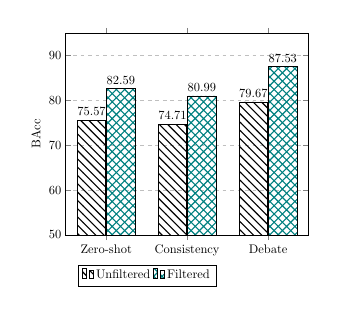
\begin{tikzpicture}[scale=0.45]
    \begin{axis}[
       ybar=2*\pgflinewidth,
        bar width=0.8cm,
        ymajorgrids = true,
        grid style=dashed,
        % xlabel={batch size},
        % title=Causality,
        ylabel={BAcc},
        nodes near coords,
        symbolic x coords={Zero-shot,Consistency,Debate},
        xtick = data,
        scaled y ticks = false,
        enlarge x limits=0.25,
        ymin=50,
        ymax=95,
        legend columns=2,
        legend style={at={(0.05,-0.15)},anchor=north west},
    ]
    

    \addplot[style={black,pattern color=black,pattern = north west lines}]
    coordinates {(Zero-shot,75.57)(Consistency,74.71)(Debate,79.67)};
    
    \addplot[style={black,pattern color=teal,pattern = crosshatch}]
    coordinates {(Zero-shot,82.59)(Consistency,80.99)(Debate,87.53)};
    


\addlegendentry{Unfiltered}
\addlegendentry{Filtered}



    \end{axis}
\end{tikzpicture}
% \vspace{-1.8em}
\end{minipage}\hspace{0.1em}
\begin{minipage}{0.23\textwidth} \centering
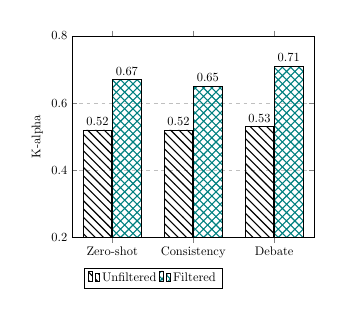
\begin{tikzpicture}[scale=0.45]
    \begin{axis}[
       ybar=2*\pgflinewidth,
        bar width=0.8cm,
        ymajorgrids = true,
        grid style=dashed,
        %xlabel={batch size},
        % title=Informativeness,
        ylabel={K-alpha},
        % ylabel shift=+60pt
        nodes near coords,
        symbolic x coords={Zero-shot,Consistency,Debate},
        xtick = data,
        scaled y ticks = false,
        enlarge x limits=0.25,
        ymin=0.2,
        ymax=0.8,
        legend columns=2,
        legend style={at={(0.05,-0.15)},anchor=north west},
    ]
    

    \addplot[style={black,pattern color=black,pattern = north west lines}]
    coordinates {(Zero-shot,0.52)(Consistency,0.52)(Debate,0.53)};
    
    \addplot[style={black,pattern color=teal,pattern = crosshatch}]
    coordinates {(Zero-shot,0.67)(Consistency,0.65)(Debate,0.71)};
    


\addlegendentry{Unfiltered}
\addlegendentry{Filtered}
\end{axis}
\end{tikzpicture}
% \vspace{-1.8em}
\end{minipage}\hfill

\caption{BAcc and correlation to human judgements results pre (black) and post (teal) filtering the ambiguous cases on annotated MeetingBank dataset.}
  \label{plot:ambiguity-filtering}
\end{figure}
\paragraph{How ambiguous cases can affect the evaluators performance?}
As can be seen from Table \ref{tab:llama-main}, even the best performing evaluators still fall very short in terms of k-alpha showing low agreement between models predictions and human annotations. Aside from the evaluators individual errors, the existence of ambiguities is a major contributing factor to low agreement and would lead to incorrect conclusions on models performance.


To remove the effect of ambiguous cases on model performance and have a more accurate estimate of evaluators performance, we filtered them out (the ones annotated as ambiguous by human annotators) from the evaluation subset (MeetingBank dataset with ambiguity annotation) and measured the performance of different models on both unfiltered/filtered data. 
As can be seen in Figure \ref{plot:ambiguity-filtering}, regardless of the setting, removing such ambiguous cases would lead to higher agreement between gold labels and the model-generated labels (with slightly larger gap for \method). Removing ambiguities can also improve FNR and FPR trends (\ref{app:results:fpr-fnr-filtered}).

% \sm{TODO currently the result here is straightforward, a more interesting result would be if removing ambiguity can result in a different model ranking, which would be important consideration for the community when evaluating evaluators}. 
% \mk{Unfortunately we don't have such results for MeetingBank. I myself annotated MediaSum and saw a flip for zero-shot VS self-consistency with and without ambiguities. Such flips can usually happen when there is not a large gap between systems in presence of ambiguities.}

% \input{tables/tab5:filtered_results_meetingbank}


\section{Conclusion}
We have proposed \method, a new automatic LLM-based multi-agent summary faithfulness evaluation with stance initialization and multi-round debate shown to be capable of identifying more errors compared to other LLM-based baselines. We have also identified a new evaluation dimension called \textit{ambiguity} and a detailed taxonomy to identify ambiguous summaries that can be evaluated as both faithful and unfaithful depending on the how one would interpret them. We extend the MeetingBank dataset by providing annotations for ambiguity dimension and show how filtering the ambiguous cases can help further improve the results and lead to higher IAA.
\section*{Limitations}
Our work has some limitations.
First, we have not used a large set of LLMs for our experiments as the primary goal of our work was to show the relative improvement of \method compared to other baseline settings with a specific LLM and how this approach can help with faithfulness evaluation regardless of the underlying LLM.
Second, our faithfulness evaluation is aimed at generating a final binary label for the non-ambiguous summaries for our choice of datasets. However, \method can be modified to ask for a faithfulness rating rather than a binary label. This can further improve the evaluation of summarizers on a finer-grained level. This can be a direction for future work.
Finally, ambiguity annotation is only done on sentence-level. More analysis is required to see whether ambiguities can span over a sentence.
% \sm{what is the IAA for the fine grained ambiguity taxonomy annotation? if it is low, it should be discussed here}.

\bibliography{custom,anthology}
\clearpage
\newpage
\appendix
\section*{Appendix}
\label{sec:appendix}
We here provide the proofs of the Propositions.


% \subsection{Proof of Proposition \ref{propo1}}
% It states that, let $\signal_1, \cdots, \signal_k$ be the signals to be corrected. Let $\sigma$ be the corresponding encoded timed word. If the timed word is accepted by the transducer of Until operator $\automaton_{p_1\until_{[a,b]}p_2}$ then  signals  satisfy $ p\until_{[a,b]}p_2$, i.e.,
%         \begin{align*}
%             \sigma \in \mathcal{L}(\automaton_{p_1\until_{[a,b]}p_2}) \implies \{\signal_1, \cdots, \signal_k\} \models p_1\until_{[a,b]}p_2
%         \end{align*}

%     Informal Proof: Let us consider the following cases based on time intervals: $[a,b), b$.
%     \begin{enumerate}
%         \item Case 1: when the time interval is $[0, a)$:\\
%         For $[0, a)$, whenever $\neg \varphi_1$ is received, the transducer modifies it and leaves $\varphi_2$ unchanged. 

%         As per the semantics of $\varphi_1\until_{[a,b]}\varphi_2$ of STL, $\varphi_1$ should be continuously true till $a$, which is ensured by the transducer.

%         \item Case 1: when the time interval is $[a,b)$:\\
%         For $[a,b)$, whenever $\neg \varphi_1$ is received, the transducer modifies it and leaves $\neg \varphi_2$ unchanged. However, if $\varphi_2$ is received, it goes to accepting location $l_2$.
        
%         As per the semantics of $\varphi_1\until_{[a,b]}\varphi_2$ of STL, $\varphi_1$ should be continuously true between $a$ and $b$. Also, if $\varphi_2$ is received the STL formula is satisfied. This is ensured by the transducer.

%         \item Case 2: when the time point is $b$:\\
%         For $b$, whenever $\neg \varphi_1$ is received, the transducer modifies it. If $\varphi_2$ is received the STL formula is satisfied. However, if $\varphi_2$ has not been received, the transducer sets $\varphi_2$ to true.

%         As per the semantics of $\varphi_1\until_{[a,b]}\varphi_2$ of STL, if $\varphi_2$ should be true at any time point between $a$ and $b$. Thus, if $\varphi_2$ is not received so far, the transducer sets $\varphi_2$ to be true. 
%     \end{enumerate}

   
% %%%%%%%%%%%%%%%%%%%%%%%%%%%%%%%%%%%%%%%%%%%%%%%%%%%%%%%%
% \subsection{Proof of Proposition \ref{propo2}}
% It states that, let $\signal_1, \cdots, \signal_k$ be the signals to be corrected. Let $\sigma$ be the corresponding encoded timed word. If the timed word is accepted by the transducer of Release operator $\automaton_{\varphi_1\release_{[a,b]}\varphi_2}$ then  signals  satisfy $ \varphi_1\release_{[a,b]}\varphi_2$, i.e.,
%         \begin{align*}
%             \sigma \in \mathcal{L}(\automaton_{\varphi_1\release_{[a,b]}\varphi_2}) \implies \{\signal_1, \cdots, \signal_k\} \models \varphi_1\release_{[a,b]}\varphi_2
%         \end{align*}
%     Informal Proof: Let us consider the following cases based on time intervals: $[0, a), [a,b), b$.
%     \begin{enumerate}
%         \item Case 1: when the time interval is $[0, a)$:\\
%         For $[0, a)$, whenever $\varphi_1$ is received, the transducer transitions to accepting location. It leaves $\neg \varphi_1$ unchanged. 

%         As per the semantics of $\varphi_1\release_{[a,b]}\varphi_2$ of STL, the formula is satisfied if $\varphi_1$ is received, which is actually modelled by the transducer.

%         \item Case 2: when the time interval is $[a,b)$:\\
%         For $[a,b)$, again whenever $\varphi_1$ is received, the transducer transitions to accepting location. If $\neg \varphi_1$  is received, the transducer modifies it.
        
%         As per the semantics of $\varphi_1\release_{[a,b]}\varphi_2$ of STL, the formula is satisfied if $\varphi_1$ is received, which is modelled by the transducer. And $\varphi_2$ should be continuously true between $a$ and $b$. This is also ensured by the transducer.

%         \item Case 3: when the time point is $b$:\\
%         For $b$, again whenever $\varphi_1$ is received, the transducer transitions to the accepting location. However, if $\neg \varphi_1$ or $\neg \varphi_2$ is received, the transducer modifies it.

%         As per the semantics of $\varphi_1\release_{[a,b]}\varphi_2$ of STL, $\varphi_1$ should be true at any time point between $a$ and $b$. Thus, if $\varphi_1$ is not received so far, the transducer sets $\varphi_1$ to be true at $b$. 
%     \end{enumerate}


%%%%%%%%%%%%%%%%%%%%%%%%%%%%%%%%%%%%%%%%%%%%%%%%%%
\subsection{Proof of Proposition \ref{propo1}}
It states that, if a timed word $\sigma$ is accepted by the transducer of Until operator $\automaton_{p_1\until_{[a,b]}p_2}$ then the corresponding signals $\signal$ satisfy $ p\until_{[a,b]}p_2$, i.e.,
        \begin{align*}
            \sigma \in \mathcal{L}(\automaton_{p_1\until_{[a,b]}p_2}) \implies \signal \models p_1\until_{[a,b]}p_2
        \end{align*}

    Proof: Let us consider the following cases based on the events received in time intervals: $[0, a], (a,b]$.
    \begin{enumerate}
        \item Case 1: when the time interval is $[0,a]$:\\
        Based on the events received at $t\in [0,a]$, we have the following sub-cases:
        \begin{enumerate}
            \item Case 1a: $p_1$ is continuously received by the transducer at $t \in [0,a]$ and $p_2$ is received at $t\in[a,a]$.

            The sequence of locations visited by the transducer for this case will be $l_0, l_1, l_2$. Thus, we see that the final location $l_2$ is reached by the transducer, thus $\sigma \in \mathcal{L}(\automaton_{p_1\until_{[a,b]}p_2})$.

            According to the semantics of STL, if $p_2$ is received at $t\in[a, a]$ until that $p_1$ is continuously received, then the STL formula is satisfied by the signals corresponding to $\sigma$. Thus the proposition holds.
            
            \item Case 1b: $p_1$ is not true at $t \in [0,a]$ and $p_2$ is true at $t\in[a,a]$.

            The sequence of locations visited by the transducer for this case will be $l_0, l_1, l_2$. On the way, the transducer modifies the signals $\signal$ to $\signal'$  such that $\signal$ is minimally modified to $\signal'$ (i.e., $min(|\signal'-\signal|))$ and  proposition $p_1$ evaluates to true for $\signal'$ (i.e., $p_1(\signal')=true$). The final location $l_2$ is reached by the transducer, thus $\sigma \in \mathcal{L}(\automaton_{p_1\until_{[a,b]}p_2})$.

            Since after modifying signals by the transducer, $p_1$ is true until $p_2$ is received at $t\in[a, a]$, thus according to the semantics of STL, the STL formula is satisfied and the proposition holds.\\
            
        \end{enumerate}
        \item Case 2: when the time interval is $(a,b]$:\\
         Based on the events received at $t\in (a,b]$, we have the following sub-cases:
        \begin{enumerate}
            \item Case 2a: $p_2$ is received by the transducer at $t \in (a,b]$ and $p_1$ is continuously received until that.
            
            The sequence of locations visited by the transducer for this case will be $l_0, l_1, l_3, l_2$. Thus, we see that the final location $l_2$ is reached by the transducer, thus $\sigma \in \mathcal{L}(\automaton_{p_1\until_{[a,b]}p_2})$.

            According to the semantics of STL, if $p_2$ is received at $t\in (a,b]$ until that $p_1$ is continuously received, then the STL formula is satisfied by the signals corresponding to $\sigma$. Thus the proposition holds.

            \item Case 2b: $p_1$ is true at $t \in 
            (a,b]$ and $p_2$ is not true at $t\in(a,b]$.

            The sequence of locations visited by the transducer for this case will be $l_0, l_1, l_2, l_3$. The transducer modifies the signals $\signal$ to $\signal'$  at $t \in [b,b]$ such that $\signal$ is minimally modified to $\signal'$ (i.e., $min(|\signal'-\signal|))$ and  proposition $p_2$ evaluates to true for $\signal'$ (i.e., $p_2(\signal')=true$). The final location $l_2$ is reached by the transducer, thus $\sigma \in \mathcal{L}(\automaton_{p_1\until_{[a,b]}p_2})$.

            Since after modifying signals by the transducer, $p_2$ is true at $t \in [b,b]$ and until that $p_1$ is true at $t\in (a,b]$, thus according to the semantics of STL, the STL formula is satisfied and the proposition holds.

             Case 2c: $p_1$ and $p_2$ is not true at $t\in(a,b]$.

             The sequence of locations visited by the transducer for this case will be $l_0, l_1, l_2, l_3$. On the way, the transducer modifies the signals $\signal$ to $\signal'$  at $t \in (a,b])$ such that $\signal$ is minimally modified to $\signal'$ (i.e., $min(|\signal'-\signal|))$ and  proposition $p_1$ evaluates to true for $\signal'$ (i.e., $p_1(\signal')=true$). Also, the transducer modifies the signals $\signal$ to $\signal'$  at $t \in [b,b]$ such that $\signal$ is minimally modified to $\signal'$ (i.e., $min(|\signal'-\signal|))$ and  proposition $p_2$ evaluates to true for $\signal'$ (i.e., $p_2(\signal')=true$).              
             The final location $l_2$ is reached by the transducer, thus $\sigma \in \mathcal{L}(\automaton_{p_1\until_{[a,b]}p_2})$.

             Since after modifying signals by the transducer, $p_2$ is true at $t \in [b,b]$ and until that $p_1$ is true at $t\in (a,b]$, thus according to the semantics of STL, the STL formula is satisfied and the proposition holds.
        \end{enumerate}
    \end{enumerate}
A similar proof can be given for the Release operator of STL and its transducer.
%%%%%%%%%%%%%%%%%%%%%%%%%%%%%%%




\subsection{Proof of Proposition \ref{propo3}}
It states that, if signals  satisfy the Until formula $ \varphi_1\until_{[a,b]}\varphi_2$, then its encoded word is accepted by its transducer, i.e., 
    \begin{align*}
        \signal \models \varphi_1\until_{[a,b]}\varphi_2 \implies \sigma \in 
        \mathcal{L}(\automaton_{\varphi_1\until_{[a,b]}\varphi_2}) 
    \end{align*}

    Proof: Let us consider the following cases based on the events received in time intervals: $[0, a], (a,b]$.
    \begin{enumerate}
        \item Case 1: when the time interval is $[0,a]$: an STL formula is satisfied at $t\in [0, a]$ by signals $\signal$, if $p_1$ of the encoded word $\sigma$ of $\signal$ is continuously true and $p_2$ of the encoded word $\sigma$ of $\signal$ is true at $t\in[a, a]$.

        For the encoded word $\sigma$ of signals $\signal$, the transducer makes a sequence of transitions involving locations $l_0, l_1, l_2$ and goes to the accepting state $l_2$. Thus,  $\sigma \in 
        \mathcal{L}(\automaton_{\varphi_1\until_{[a,b]}\varphi_2})$. and proposition holds.

        \item  Case 2: when the time interval is $(a,b]$: an STL formula is satisfied at $t\in (a,b]$ by signals $\signal$, if $p_2$ of the encoded word $\sigma$ of $\signal$ is received at $t\in (a,b]$ and  $p_1$ of the encoded word  $\sigma$ of $\signal$  is continuously true until that.

        For the encoded word $\sigma$ of signals $\signal$, the transducer makes a sequence of transitions involving locations $l_0, l_1, l_3, l_2$ and goes to the accepting state $l_2$. Thus,  $\sigma \in 
        \mathcal{L}(\automaton_{\varphi_1\until_{[a,b]}\varphi_2})$. and proposition holds.
    \end{enumerate}

A similar proof can be given for the Release operator of STL and its transducer.









\end{document}


% Multi-Agent Debate with Initial Stance
% MADIS

% Multi-Agent Debate with initial stance and AMbiguity detection
% MADAM

% Multi-Agent Debate with Initial Stance and Abiguity detectioN
% MADISON